\documentclass[12pt]{article}
\usepackage[a4paper,margin=1in,footskip=0.25in]{geometry} % set margins
\usepackage[portuguese]{babel}
\usepackage[utf8]{inputenc}
\usepackage[hidelinks]{hyperref} 
\usepackage{amsmath}
\usepackage{amssymb}
\usepackage{amsthm}
\usepackage{graphicx}    % needed for include graphics
\usepackage{subfigure}   % add subfigures
\usepackage{indentfirst}
\usepackage{float}       % needed for [H] figure placement option
\usepackage{setspace}    % needed for doublespacing
\usepackage{tikz}
\usepackage{algpseudocode}
\usepackage{listings}
\usepackage{xcolor}

\definecolor{mGreen}{rgb}{0,0.6,0}
\definecolor{mGray}{rgb}{0.5,0.5,0.5}
\definecolor{mPurple}{rgb}{0.58,0,0.82}
\definecolor{backgroundColour}{rgb}{0.95,0.95,0.92}

\lstdefinestyle{CStyle}{
    backgroundcolor=\color{backgroundColour},   
    commentstyle=\color{mGreen},
    keywordstyle=\color{magenta},
    numberstyle=\tiny\color{mGray},
    stringstyle=\color{mPurple},
    basicstyle=\footnotesize,
    breakatwhitespace=false,         
    breaklines=true,                 
    captionpos=b,                    
    keepspaces=true,                 
    numbers=left,                    
    numbersep=5pt,                  
    showspaces=false,                
    showstringspaces=false,
    showtabs=false,                  
    tabsize=2,
    language=C
}

% Macros
\renewcommand{\familydefault}{\sfdefault} % sans-serif
\newcommand{\lowtext}[1]{$_{\text{#1}}$}
\newcommand{\code}[1]{\texttt{#1}}

% Adds ./img/ to the path of figures
\graphicspath{{./img/}}

\title{Relatório EP3 - MAC0219}
\author{Bruno Sesso, Gustavo Estrela de Matos, Lucas Sung Jun Hong}

\begin{document}
% Espaçamento duplo 
\doublespacing
\begin{titlepage}
    \vfill
    \begin{center}
        \vspace{0.5\textheight}
        \noindent
        Instituto de Matemática e Estatística \\
        EP3 - MAC0219 \\
        \vfill
        \noindent
        {\Large Cálculo do Conjunto de Mandelbrot
        em Paralelo com OpenMPI} \\
        \bigskip
        \bigskip
        \begin{tabular}{ll}
            {\bf Professor:} & {Alfredo Goldman} \\
            {\bf Alunos:}    & {Bruno Sesso} \\
                             & {Gustavo Estrela de Matos} \\
        \end{tabular} \\
        \vspace{\fill}
       \bigskip
        São Paulo, \today \\
       \bigskip
    \end{center}
\end{titlepage}

\pagebreak
\tableofcontents
\pagebreak

\section{Introdução}
Neste trabalho, implementaremos uma versão paralela, em OpenMPI, do 
código que calcula o fractal de uma região de Mandelbrot. Esta versão
deve ser capaz de, dado um cluster de computadores, utilizar o padrão
de troca de mensagens MPI para distribuir e reunir em um nó principal
os cálculos necessários para gerar a imagem da região pedida.

Ao longo desse trabalho, iremos apresentar resultados de tempo de 
execução das diferentes implementações e suas respectivas variações.
Para isso, utilizamos a ferramenta {\em perf}, capaz de realizar 
repetições de experimentos, apresentando resultados médios e com desvio
padrão. Todos os resultados apresentados aqui foram feitos a partir de
no mínimo 10 execuções do mesmo comando.
        

%%%%%%%%%%%%%%%%%%%%% SEQUENCIAL %%%%%%%%%%%%%%%%%%%%%%%%%%%%%%
\newpage
\section{Código Sequencial}
O código sequencial foi fornecido no enunciado do EP e com ele fizemos
medições de tempo para diferentes regiões do plano complexo.

\begin{figure}[H]
    \makebox[\textwidth][c]{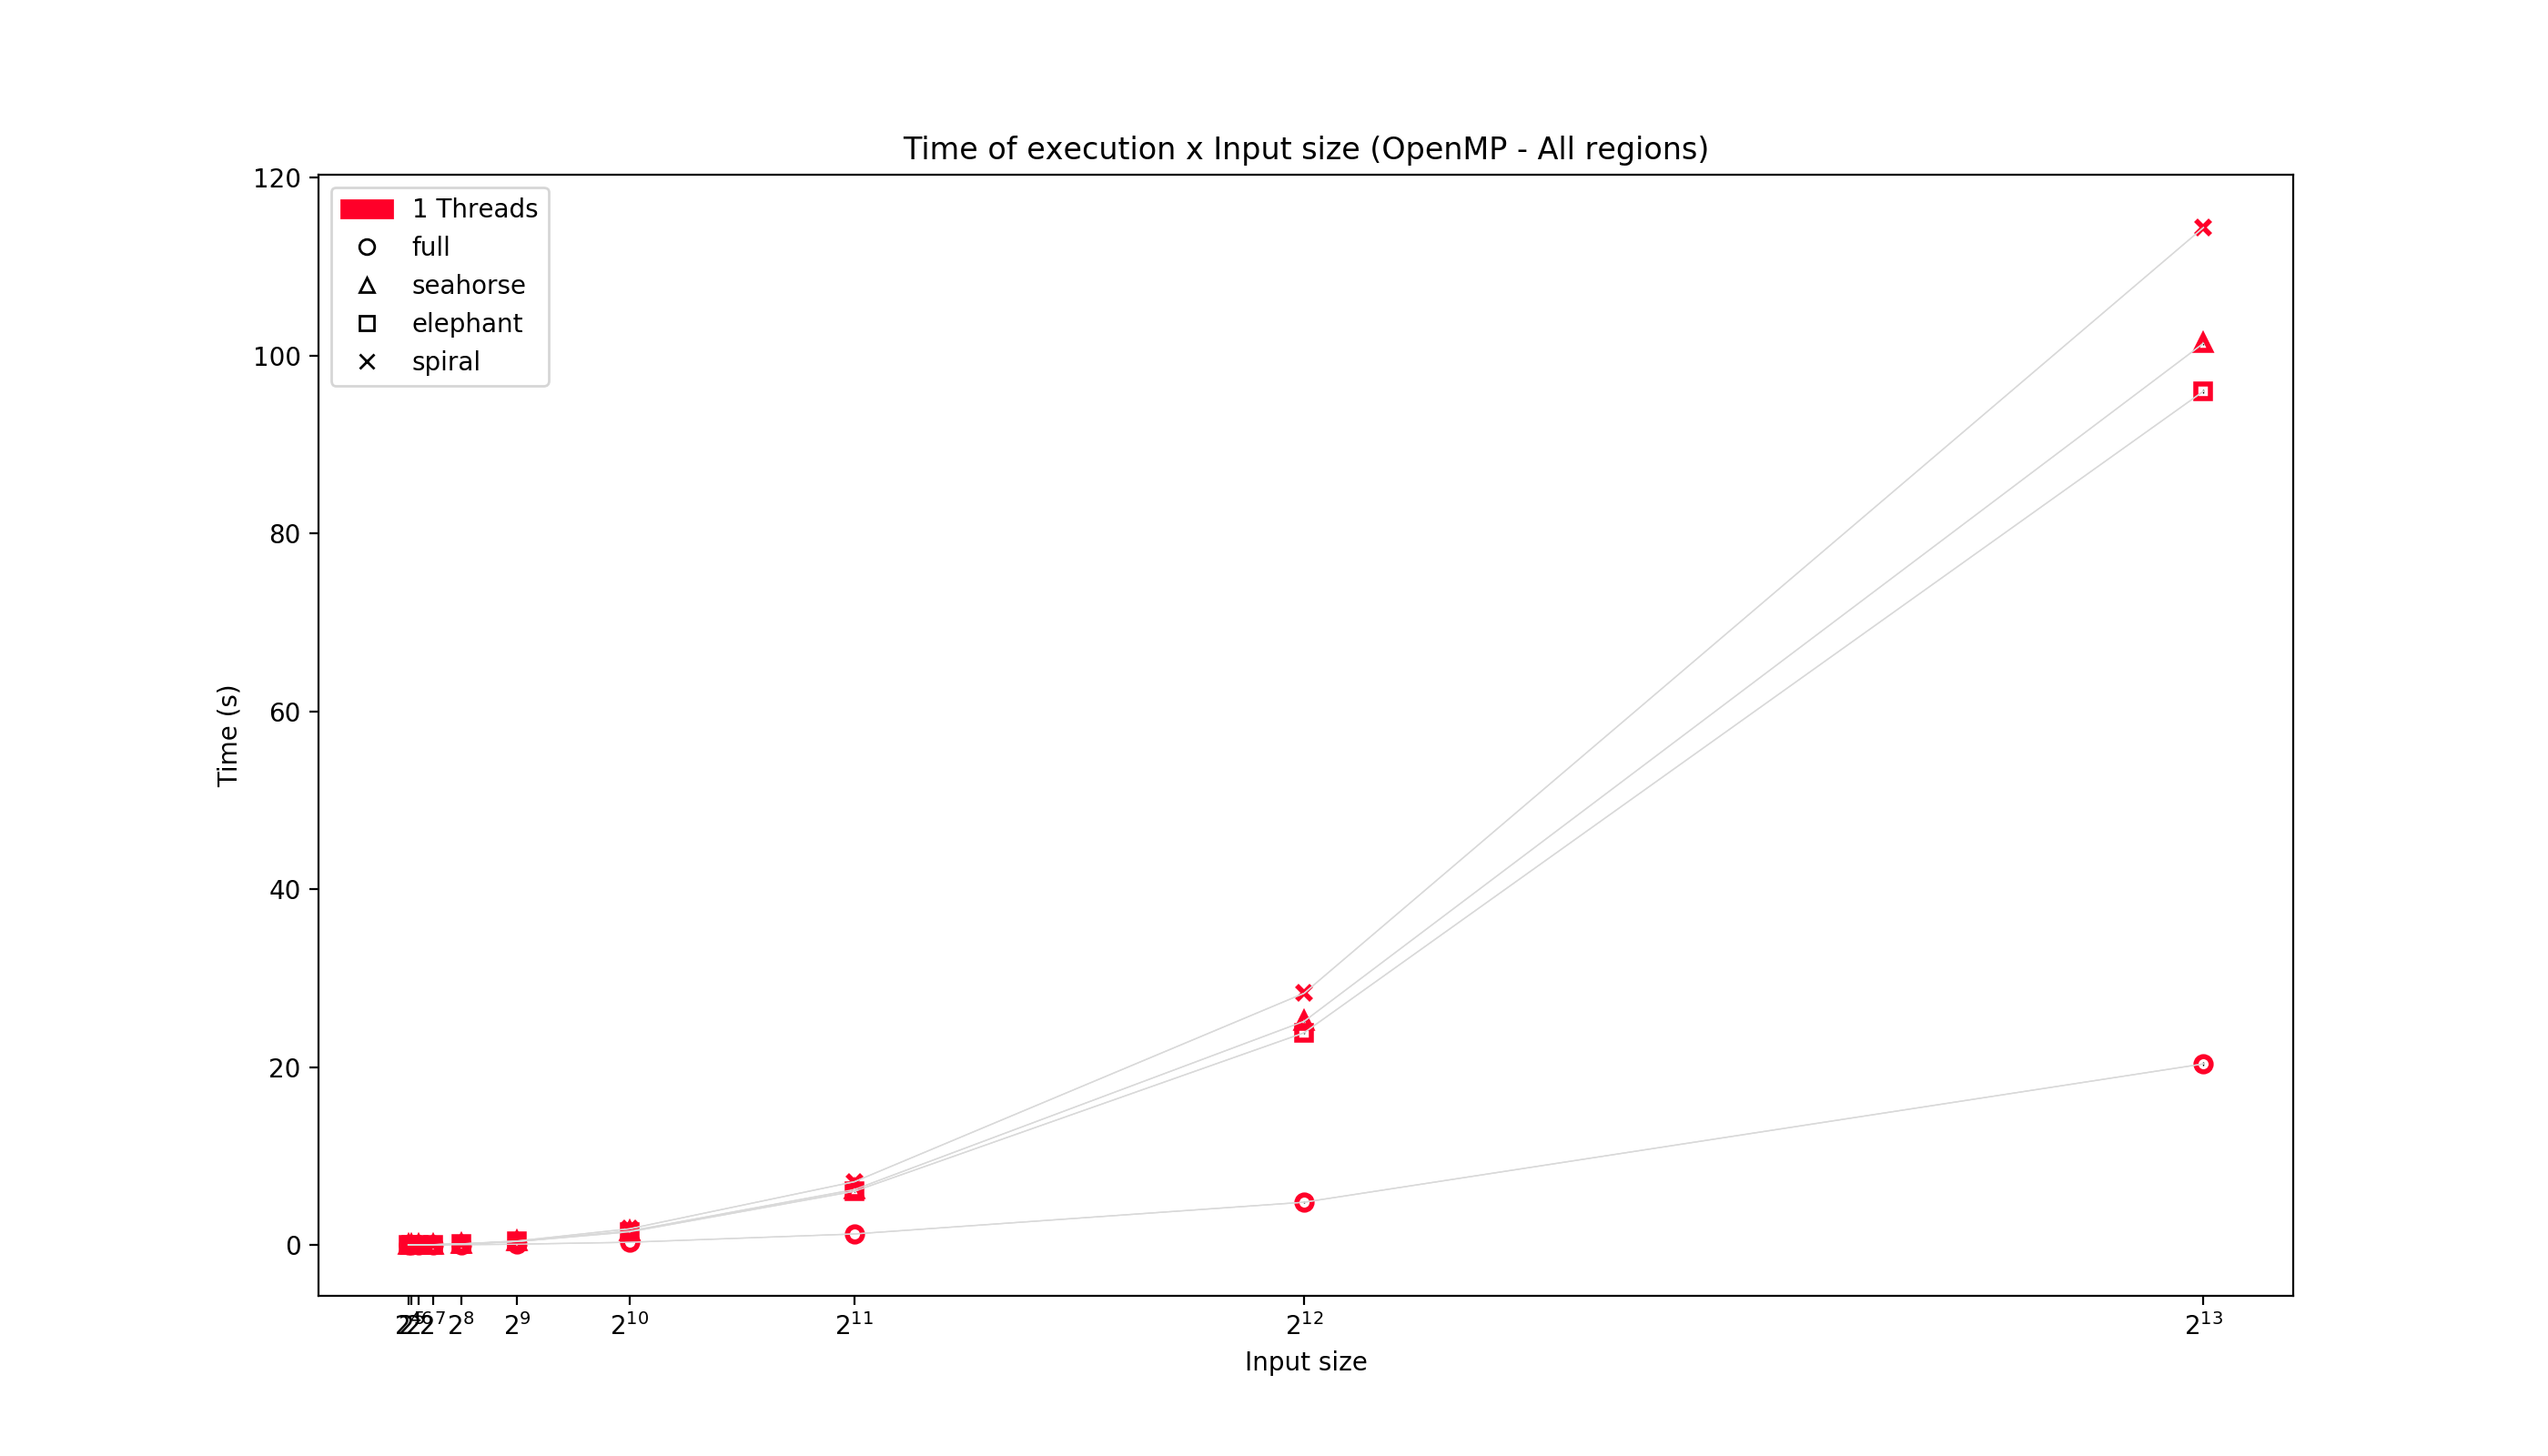
\includegraphics[scale=.50]{seq_with/all_timeXsize_OpenMPpng.png}}
    \caption{Tempo de execução do programa sequencial para diferentes 
    tamanhos de entrada}
\end{figure}

Nota-se que o tempo em cada região é diferente, pois em cada região
pode haver mais cálculos de pontos com mais interações. Em especial, 
podemos observar que a região Full é a mais fácil de ser calculada.

Como explicamos no EP1, o cálculo dessas regiões escala de uma maneira,
aparentemente, mais do que linear. Além disso, o consumo de tempo 
causado por operações de alocação, leitura e escrita de memória são 
lineares e serão desconsideradas nesse trabalho.



%%%%%%%%%%%%%%%%%%%%% OPENMPI %%%%%%%%%%%%%%%%%%%%%%%%%%%%%%
\newpage
\section{Código em OpenMPI}
A nossa implementação em OpenMPI define uma máquina como principal 
(mestre), e esta deve ser capaz de dividir o trabalho entre as outras 
máquinas (escrava), assim como reunir os resultados para construir a 
imagem da região Mandelbrot. Para fazer isso, dividimos os pontos da 
imagem em blocos de pixels e, então a máquina principal envia para 
outras máquinas os blocos que devem ser calculados, por meio de uma 
mensagem que indica o índice do bloco que deve ser calculado. Depois de
calcular o bloco, a escrava envia para mestre um vetor que contém as
iterações calculadas naquele bloco para compor a imagem.

A estrutura de blocos que usamos neste trabalho é a mesma usada no EP1 
e, como fizemos na última vez, vamos dividir a imagem em $n$ blocos, em
que $n$ é o tamanho do lado da imagem, isto é, cada bloco corresponde a
uma linha da imagem. Além disso, como constatamos no EP1 que uma divisão
dinâmica de trabalho é mais vantajosa, vamos adotar essa abordagem 
também neste trabalho. Ao invés de pré-determinar em qual máquina um
bloco será calculado, delegamos a máquinas livres blocos que ainda não
foram calculados.

Para implementar essa divisão dinâmica de trabalho, a máquina mestre 
deve iniciar o processo delegando um bloco para cada máquina escrava.
Depois, sempre que uma máquina enviar o trabalho pronto, a mestre deve
processar essa resposta, atualizando o buffer da imagem, e enviar a
escrava um novo bloco para ser calculado (se houver). Para finalizar o
processo, a mestre também deve enviar um sinal de "trabalho feito" para
todas escravas, o que faz possível terminar o programa em todas as 
máquinas do cluster.

Veja abaixo um pseudo-código da função que roda na máquina mestre, 
distribuindo os blocos de pixels para as máquinas escravas:
\begin{algorithmic}[1]
\Function{DistributeWork}{}
    \State $S \gets $ lista de nacos de todos os pixels
    \State $sent\_chunks \gets 0$
    \State $received\_chunks \gets 0$ 
    \ForAll{$M$ máquina escrava do cluster}
        \State $Send (M, S[sent\_chunks])$
        \State $sent\_chunks \gets sent\_chunks + 1$
    \EndFor
    \While{$received\_chunks < |S|$}
        \State $N \gets PullJobFromAnyMachine ()$
        \Comment{Recebe trabalho de escrava N}
        \State $received\_chunks \gets received\_chunks + 1$
        \If{$sent\_chunks < |S|$}
            \State $Send (N, S[sent\_chunks])$
            \State $sent\_chunks \gets sent\_chunks + 1$
        \Else
            \State $Send (N, END\_CODE)$
        \EndIf
    \EndWhile
\EndFunction
\end{algorithmic}

\newpage
\section{Conclusão}

\newpage

\end{document}
